\documentclass{article}
\usepackage{graphicx}
\begin{document}

\title{5611 HW3: The Travelling Salesman Problem}
\author{Shane Harding \\ 10309405}

\maketitle

\section{Introduction}

This report details everything that I did in this assignment and why I did things the way I did.

\section{Task 1}

There are multiple C files to this task that are then all compiled together via the makefile.

The first thing I did was write a function that computes the distance between two points on a two dimensional plane (written in \verb!dist.c!). This does not give the proper Euclidean distance since I do not compute the square root (just $x^2 + y^2$ is calculated). The reason for this is that square root calculations are expensive and not necessary in this case. They aren't necessary because we are just comparing distances and if $d_1^2$ is bigger than $d_2^2$ then $d_1$ is bigger than $d_2$.

In my main file, the first thing I do is deal with the command line arguments and flags. So only one or zero flags are allowed. If there are no flags then the number of cities is simply set to 10. The \verb!-f! flag allows for a configuration of cities to be loaded from a specified file. The \verb!-n! flag generates a specified number of random cities on a grid.

Once all the coordinates of the cities are loaded/generated a distance matrix is set up. This puts the distance between cities $i$ and $j$ in the matrix entry $(i,j)$. The initial ordering of the cities set to be $0,1,...,n-1$. The permutation function is then called to generate all the possible routes. At this stage it is important to note that I am solving this problem for closed paths. So the first point and the last point are connected. This means that our starting city does not make any difference (because the path taken is always going to be a closed loop). Which then means that we don't have to move it in our permutations. And we also have $(n-1)!$ possible paths.

There is a swap function that simply swaps two elements in an array. This is needed in my function that generates all the permutations of the $n$ cities. The permutation function writes all of the permutations to a file. The reason for this is that the permutation function is called recursively within itself. This made returning a value from it very difficult and I found it much easier to just write all the permutations to a file and then read them from the file when they were required.

Also, since I wrote to the file and then wanted to read from it. It meant that I had to close if and open it again, because I couldn't find a way to just open it in both read and write mode; it had to be one or the other.

Once all the possible permutations (routes) are read, the distances of each is calculated (by simply adding the relevant elements of the distance matrix) and the shortest one is returned. This is done in the \verb!shortest_route.c! function. The shortest path is then printed to the terminal. And all the mallocs are then freed.

\section{Task 2}

The times for a solution to be obtained as a function of the number of cities is shown in the figure.

\begin{figure}
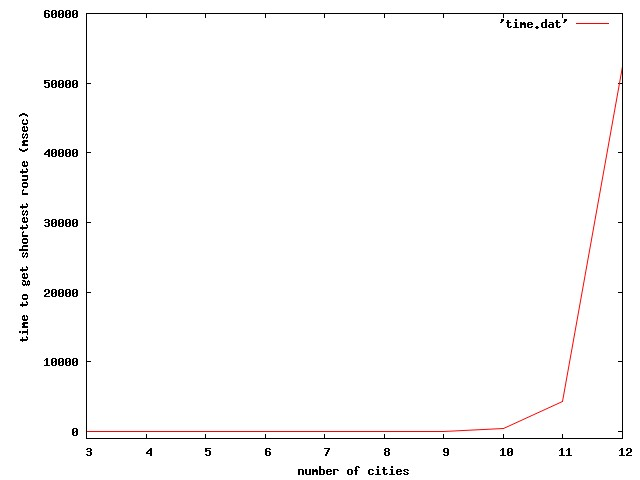
\includegraphics[scale=0.5]{../task2/plot.jpg}
\caption{This figure shows the time taken to compute the solution as a function of the number of cities.}
\end{figure}

From this figure we can see how the computation time grows rapidly with the increase in the number of cities. We can see how the time taken obeys the rule $t_{n+1} = t_n c_n$. Where $t_{n+1}$ is the time for the next step (presuming $t_n$ is the time for the current step) and $c_n$ is the number of cities in the current step. From this we can see that $t_{n+1}=c_n c_{n-1} t_{n-1}$ and then continuing this we see $t_{n+1} = c_n ... c_0 t_0 = c_n ! t_0$. So if we take $t_10 = 390$ with $n=10$ then we see that $t_20 = \frac{19!}{10!}t_{10}$, so $t_{10}=1.3 \times 10^{13}$. And similarly we find that $t_50=6.6 \times 10^{58}$ and $t_100 = 1.0 \times 10^{152}$. All times are in msecs.

\section{Task 3}

For this I edited my code to work with the file format similar to \verb!att48.tsp!. This just involved changing how the file was read to skip the first six lines of the file and read in the coordinates correctly.

I then tried to implement an nearest neighbour algorithm to solve the problem heuristically. This method involves choosing a point to start from at random. The next city is then chosen as simply whichever one is closest. Then then next city is the one that is closest and hasn't been visited yet. This process is then repeated until all the cities are visited. I tried to implement this with a linked list to keep track of the cities that had yet to be visited. But ran into difficulties and couldn't get it to work fully.

\section{Task 4}

The TSP is a very difficult problem to parallise, and the speedup when it has been parallised isn't great and it doesn't scale well at all. The brute force approach can be trivially parallised using the master slave, by giving each proc a different path to calculate but this doesn't really give too much of a performance boost. However, some of the heuristic methods are more friendly to being parallelised, in particular the genetic algorithm. The genetic algorithm can be effictively parallised and things like genetic mutations would help to prevent the solution getting stuck in a local minimum, which happens in many of the methods that only find an optimal solution and not the best solution.



\end{document}
